
\chapter{Script-level Functionalities} \label{chap:script}
Now that the Event Engine is raising MPTCP events, we can start using them in order to track MPTCP behavior on the network. This section will describe the problems we have tackled. We will explain why it is useful and describe how we can use Bro's script interpreter to showcase certain actions.

\section{Logging MPTCP Connections} \label{section:mp log}
Logging is one of Bro's main features. Logs are important in a great number of cases. They can be used for forensic analysis to determine if an attack took places, for network or protocol performance evaluations, or even to look for traffic trends or understand user behavior. With our new MPTCP events, we will try to log MPTCP traffic specifically. The \texttt{conn.log} is a log the Bro creates by default to log the different end-to-end connections that appear over the network. A quick examination of this log shows that it contains a lot of useful information, such as the transport layer protocol used, the duration of the connection, and the number of packets that were exchanged. Since this information is already available, we will concentrate on what is not, and more importantly, on what is unique to MPTCP. \\

Obviously, we will want to find each TCP connection that was used as an MPTCP subflow. Each one will be identified by the four-tuple that usually defines a connection: the address and port of both endpoints. Next, we will want to group TCP connections that belong to the same MPTCP connection. To do this, we will uniquely identify each MPTCP connection and add a column to the log indicating which MPTCP connection each subflow belongs to. Finally, we might want to know whether a given TCP subflow was the original subflow of its MPTCP connection or not. We will therefore add a column of booleans to show this. \\

In order to do the logging, we will of course use the logging framework that we discussed in section \ref{section: logging}. Since we have decided what information we wish to log, we can redefine the \texttt{Log::ID} constant and create our custom \texttt{Info} record like so: \\

\begin{code}	
	type Info: record {
		orig_h:			addr &log;
		orig_p:			port &log;
		resp_h:			addr &log;
		resp_p:			port &log;
		isOrig:			bool &log;
		MP_ID:			count &log;		
	};
\end{code}

Where \texttt{orig} and \texttt{resp} stand for the connection's initiator and responder, \texttt{h} is for the address, \texttt{p} is for the port. \texttt{isOrig} is the boolean specifying if the connection is the first one of the MPTCP connection, and \texttt{MP\_ID} is the MPTCP connection's unique identifier. This record will give us the log header shown in figure \ref{pic:log header}. \\

\begin{figure}[!t]
\centering
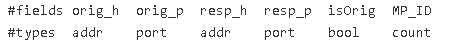
\includegraphics[scale = 0.7]{Figures/logheader.png}
\caption{Header for our MPTCP connection log}
\label{pic:log header}
\end{figure}

After creating the log stream, all we have left to do is create the log entries. Traditionally for TCP, Bro considers a connection established starting from the SYN+ACK response in the three-way handshake. Barring aborted connections or failed authentication, which deserves its own special treatment, we can use the same assumption for our subflows. Therefore, a new subflow will be considered set up in two cases: \\

\begin{enumerate}
\item When we see an MP Capable option of length 12 from the responder of the connection.
\item When we see an MP Join option of length 16.
\end{enumerate}

As a reminder, MP Capable options are of length 12 for both the SYN and SYN+ACK since they only carry one 8-byte key, and length 20 on the final ACK since they carry both keys. The two cases where they have a length of 12 can be differentiated by using the \texttt{is\_orig} boolean that is sent in the \texttt{mp\_capable} event. MP Join options have different length at each step, 16 being the length of the SYN+ACK since it carries the truncated HMAC for the authentication process (8 bytes), and the responder's random number (4 bytes). \\

The first case is the simplest. Since the connection is using an MP Capable option, it means that the hosts are establishing a new MPTCP connection. Our \texttt{mp\_capable} event handler can therefore create a new log entry immediately. The addresses and ports can be extracted by the \texttt{connection} record which is sent with the event. \texttt{isOrig} will always be true in this case since the MPTCP has just been created. For the final field, \texttt{MP\_ID} we simply keep a global counter which we increment at each new MPTCP connection. The value of this counter is used as the unique identifier (the Bro count type uses 64 bits which should be enough to uniquely identify connections). \\

The second case is when a new TCP connection is established using the MP Join option. The logic for this case will be written into the \texttt{mp\_join} event handler, after a guard ensuring the length of the option is 16. In this case, we are obviously facing an MPTCP connection that has already been established in another flow, \texttt{isOrig} will therefore always be false. The addresses and ports can once again be extracted from the connection record that is passed within the event. The main difficulty comes from finding which  MPTCP connection this subflow is part of. On a single host, the MPTCP implementation identifies each active connection with a 32-bit token which is sent within the MP Join option. However, Bro will be observing traffic to and from a multitude of hosts and we will not have access to each one's token-to-connection mapping. Furthermore, given two IP addresses, we cannot even tell if they both belong to the same host, whereas the host itself is obviously aware of which addresses are his. \\

In order to cope with this, we will need to re-create these mappings within the script. To do this, will make extensive use of Bro's \texttt{table} structure, a traditional key-value store. We will also define our own record types. First, we define an \texttt{MP\_host}. This data structure represent one endpoint of one MPTCP connection. Once again, Bro cannot know that two distinct MPTCP connections from different addresses come from the same physical host. Thankfully, we don't need to and we can consider each MPTCP connection to belong to two new hosts as long as we can find all the connection's subflows. The record contains the \texttt{MP\_ID} of the connection which this host belongs to, the list and number of know addresses this host has advertised and/or used (this is also the mapping between addresses and address IDs which MPTCP uses, and we will have other uses for it later), and the identifier of the other host participating in the connection. The second record we will use is the \texttt{MP\_conn} record. This data structure represents one MPTCP connection. It contains the identifiers of both \texttt{MP\_hosts} involved, as well as the number of active subflows. Finally, we define an \texttt{MP\_addr} record as simply an address and port pair. \\

The next step is creating the tables that will maintain the mappings we need. Tables are used to retrieve a value for a given key, but not the other way around. We therefore need to think about what data we will have available to use as key, and what data we will need to retrieve. When we receive an MP Join, we will have the addresses and port numbers of the TCP connection and the MPTCP token to work with. Maintaining a mapping of the tokens requires re-computing the cryptographic operations of every host, so we will avoid this for the time being. That leaves the addresses. For a host to establish a new subflow, the destination address must either be the same as that of the original subflow, or have been advertised by the other host on a known subflow of the connection. Therefore, our first table will use \texttt{MP\_address}es as keys and map them to the \texttt{MP\_host} that advertised them (or created an MPTCP connection on it). Even though the \texttt{MP\_host} contains the list of its addresses, this will not be available when we receive the Join. \texttt{MP\_host}s are referenced by unique IDs. An additional table will thus serve to map IDs to the corresponding hosts.\\

With these structures ready, we return to the \texttt{mp\_capable} event handler. When a new TCP subflow is established, we create two new \texttt{MP\_host}s representing the to endpoints of the TCP connection. Each one is made aware of the other, and originally contains only one address: the one used on the current subflow. Both these hosts are added to the hosts table. Next, both the originator and responder address/port pairs are mapped to their respective host in the address table. Now, when we receive an MP Join with length 16, we can lookup the ID of the \texttt{MP\_host} the destination address belongs to using the address table. With this ID, we use the host table to lookup the corresponding \texttt{MP\_host} which contains the ID of the \texttt{MP\_conn}. This is all the information we need in order to create the log entry. However, one issue remains: besides the addresses of the original subflow, we are not populating the address table. \\

In order to do this, we need to use the \texttt{mp\_add\_addr} event handler. Add Addr options are always sent on an existing subflow so the hosts will already be known. The first step is determining which one of the two hosts is advertising the new address. This is done simply by using the \texttt{is\_orig} value of the event. If it is true, we find the host's ID by doing a lookup with the connection originator's address in the address table. If it false, we do the lookup with the responder's address. Once the correct ID has been found, we update the address table by mapping the new address to the host ID. We also update the host's address mapping at this point. An important note is that the port number in a Add Addr option is optional. As per the RFC, if it is not provided, we  use the same port number as the one used to send the option. \\

An additional case to consider is that a host may use an address that it has not explicitly advertised to initiate a new connection. Indeed, it may send an MP Join from an unknown address to one that the other host has advertised. In order to cope with this, the \texttt{mp\_join} handler will also populate the address table of a host if the incoming address of the Join message is not known.\\

With everything in place, we can run Bro on a packet trace while loading the script, and we find a new log consistent with the format we were expecting: \\

\begin{code}
#separator \x09
#set_separator	,
#empty_field	(empty)
#unset_field	-
#path	mp__connection
#open	2015-05-30-23-36-19
#fields	orig_h	orig_p	resp_h	resp_p	isOrig  MP_ID
#types	addr	port	addr	port	bool	count
2a02:a03f:2220:4300:9009:ac68:352f:d0cc	48020	2001:6a8:308f:1:216:3eff:fec5:c815	80	T	0
192.168.1.47	48190	130.104.230.45	80	F	0
2a02:a03f:2220:4300:204:4bff:fe0a:54f9	39238	2001:6a8:308f:1:216:3eff:fec5:c815	80	F	0
2a02:a03f:2220:4300:9009:ac68:352f:d0cc	48022	2001:6a8:308f:1:216:3eff:fec5:c815	80	T	1
192.168.1.47	40568	130.104.230.45	80	F	1
2a02:a03f:2220:4300:204:4bff:fe0a:54f9	34776	2001:6a8:308f:1:216:3eff:fec5:c815	80	F	1
192.168.1.47	50760	137.110.116.31	80	T	2
192.168.1.47	50763	137.110.116.31	80	T	3
192.168.1.47	50764	137.110.116.31	80	T	4
192.168.1.47	50765	137.110.116.31	80	T	5
192.168.1.47	50775	137.110.116.31	80	T	6
192.168.1.47	50776	137.110.116.31	80	T	7
192.168.1.47	50769	137.110.116.31	80	T	8
192.168.1.47	50768	137.110.116.31	80	T	9
192.168.1.47	50770	137.110.116.31	80	T	10
192.168.1.47	50818	137.110.116.31	80	T	11
192.168.1.47	50819	137.110.116.31	80	T	12
192.168.1.47	50820	137.110.116.31	80	T	13
192.168.1.47	50820	137.110.116.31	80	T	14
192.168.1.47	50819	137.110.116.31	80	T	15
192.168.1.47	50826	137.110.116.31	80	T	16
192.168.1.47	50828	137.110.116.31	80	T	17
192.168.1.47	50827	137.110.116.31	80	T	18
192.168.1.47	50828	137.110.116.31	80	T	19
192.168.1.47	50827	137.110.116.31	80	T	20
2a02:a03f:2220:4300:9009:ac68:352f:d0cc	48178	2001:6a8:308f:1:216:3eff:fec5:c815	80	T	21
2a02:a03f:2220:4300:204:4bff:fe0a:54f9	53632	2001:6a8:308f:1:216:3eff:fec5:c815	80	F	21
192.168.1.47	58468	130.104.230.45	80	F	21
192.168.1.47	59310	178.254.13.90	80	T	22
192.168.1.47	59311	178.254.13.90	80	T	23
2a02:a03f:2220:4300:204:4bff:fe0a:54f9	53657	2002:b2fe:d5a::1	80	F	23
2a02:a03f:2220:4300:204:4bff:fe0a:54f9	49181	2002:b2fe:d5a::2	80	F	23
2a02:a03f:2220:4300:9009:ac68:352f:d0cc	33329	2002:b2fe:d5a::1	80	F	23
2a02:a03f:2220:4300:9009:ac68:352f:d0cc	54239	2002:b2fe:d5a::2	80	F	23
#close	2015-05-30-23-36-24
\end{code}

With these steps, the MPTCP connection log is functional. For performance reasons though, we still need to cleanup our data structures once they are no longer needed. In order to do this, we can use a handler for the \texttt{connection\_state\_removed} event. This event is automatically raised when the Event Engine removes a stream from its memory, usually when it is terminated. This event only provides us with the connection record of the stream being removed. If the connection is known within our script, we will remove all the data related to that connection. When removing the last subflow of an MPTCP connection, we also remove all the data related to the connection and the two hosts involved. \\

As mentioned earlier in this section, MPTCP itself uses the tokens in order to recognize which sub-flows belong to which connection. The reason for this is that, due to middle boxes such as NATs, the addresses that are advertised might not correspond to those that are observed during Joins. Since we are not computing the tokens at this time, this means that the script cannot function in the event where such modifications are taking place. While using the tokens would be an improvement, it is important to remember that they are not enough on their own. Indeed, tokens are meant to be locally unique. However,  since Bro observes traffic to and from many hosts, it is not guaranteed that the use of tokens will be collision-free.

\section{Detecting Erroneous Address Advertisement} \label{section:add addr log}
As explained in chapter \ref{chap:mptcp}, an MPTCP host maintains, for each one of its MPTCP connections, a mapping of its addresses and those of the other host to address IDs. When a new address is advertised, the mapping used by its owner is sent along in the Add Addr option. The address ID is used in place of the actual address for address removal, changes in path priority, and most importantly for joining connections. Indeed, due to NATs (Network Address Translators) and other middle boxes along the paths, the address in the packet header of an MP Join might not correspond to an address that was advertised. The address ID is therefore used to specify the address unambiguously. Our next task will be to detect if address advertisement goes wrong. Within a given MPTCP connection, an address ID should map to one and only one address/port pair. If we receive an Add Addr option with a already used ID, there are three possible cases: \\

\begin{enumerate}
\item The new address is the same as the existing one and the port is different. In this case, the host is changing the advertised port which is authorized.
\item The Add Addr is a duplicate, advertising the same address and port on a given ID. This is normally ignored.
\item The new address is different, leading to two addresses mapping to the same ID. This is not allowed and is the behavior we will want to detect.
\end{enumerate} 

When using a correct MPTCP implementation, this third case should not happen. Detection of this behavior may therefore be and indicator of an attack. For example, an attacker may have eavesdropped on an MPTCP connection and would be attempting to advertise his own addresses as being available for the connection while pretending to be one of the two legitimate hosts. While the utility of doing this may be questionable, the possibility is real. Figure \ref{pic:2 adds} shows three packets captured with Wireshark. The first is the final ACK of a connection establishment. The following two packets, while seeming like duplicates, are actually address advertisements. Figures \ref{pic:2 adds detail1} and \ref{pic:2 adds detail2} show the detailed TCP headers of both these packets. It is easy to see that, if an attacker were to sniff one, it would be easy to forge the second. The only variations are the option length (and only because one is an IPv4 address and the other is IPv6), the TCP checksum (easy to recalculate), and the advertised address and ID itself.  Figure \ref{pic:2 add attack} shows a potential scenario where an adversary observing and Add Addr would send his own advertisement as a forged duplicate of the previous packet. Should Host A ever try to perform a legitimate Add Addr on the ID the adversary chose, the IDs would clash, allowing for detection. A possible application of this attack  would consist of an attacker filling up all 254 available address IDs (8 bits, ID 0 used by the initial subflow and at least one advertised in the sniffed packet), thereby making it impossible for the connection to establish more subflows.\\

\begin{figure}[!t]
\centering
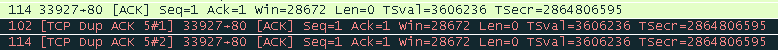
\includegraphics[scale = 0.6]{Figures/2addaddrwireshark.png}
\caption{A Three-way handshake ACK followed by two Add Addr duplicates}
\label{pic:2 adds}
\end{figure}

\begin{figure}[!t]
\centering
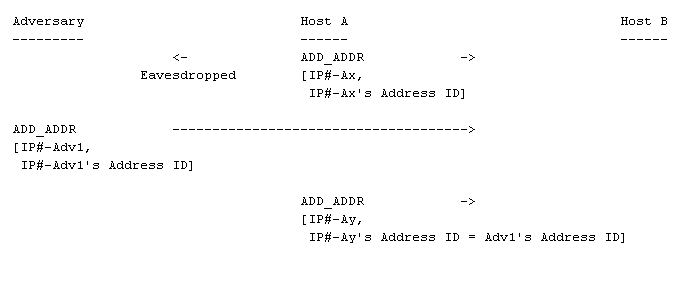
\includegraphics[scale = 0.6]{Figures/addaddrattack.png}
\caption{Possible Add Addr Attack}
\label{pic:2 add attack}
\end{figure}

\begin{figure}[!t]
\centering
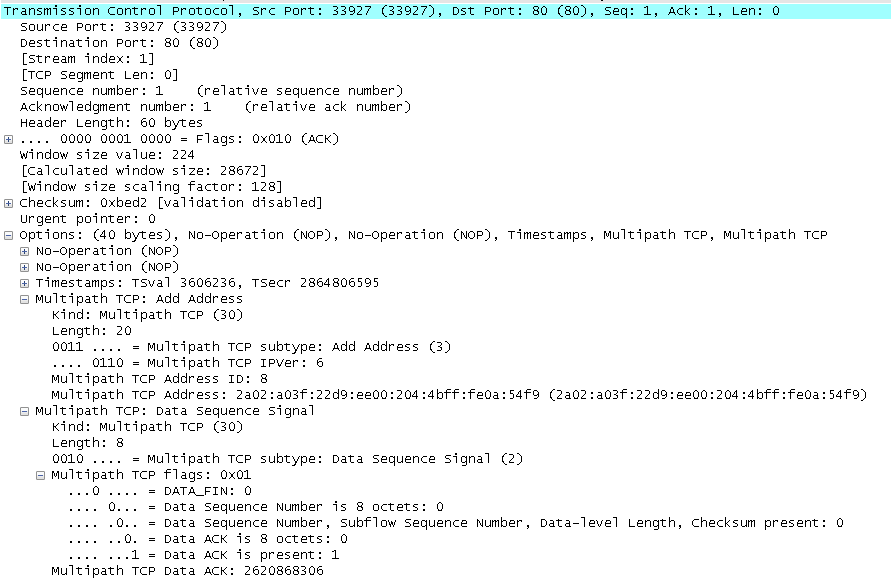
\includegraphics[scale = 0.75, angle = 90]{Figures/addaddr1.png}
\caption{The first Add Addr in detail}
\label{pic:2 adds detail1}
\end{figure}

\begin{figure}[!t]
\centering
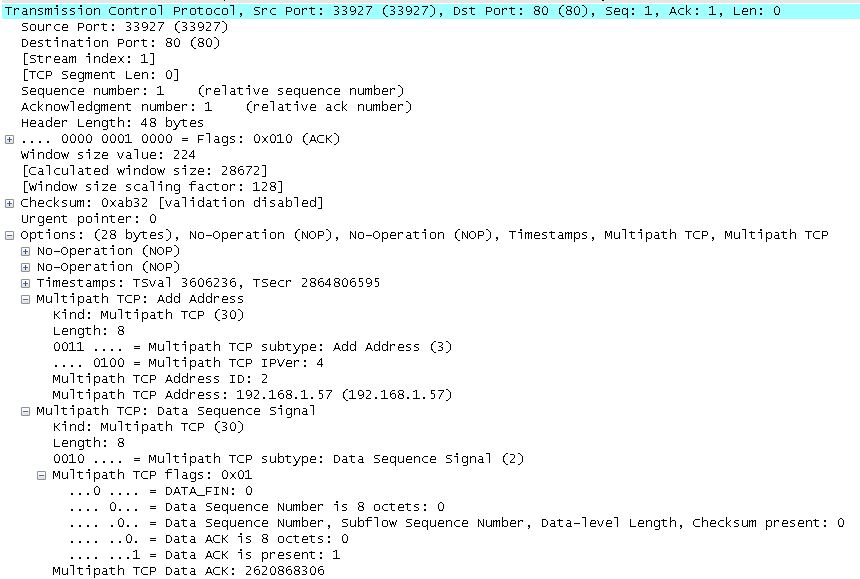
\includegraphics[scale = 0.75, angle = 90]{Figures/addaddr2.png}
\caption{The second Add Addr in detail}
\label{pic:2 adds detail2}
\end{figure}



Should this ever happen on our network, we would therefore want to be notified about it. Unlike the logging of MPTCP connections we saw in the previous section which aims at logging normal behavior, this time we are interested in abnormal cases. For an immediate response, we will therefore make use of the Notice framework described in section \ref{section: notice}. After adding our new notice type to the framework, we go back to the \texttt{mp\_add\_addr} handler, unsurprisingly. We have already used this handler to populate our address table. The first step to that process was getting the ID of host which was advertising the address. We can use this ID to lookup the host record itself in the host table. As we mentioned in the previous section, the host record maintains the mapping between its known addresses and their address IDs. This is exactly what we need, and now is the time to use it. \\

The \texttt{mp\_add\_addr} contains the address ID that is supposed to be used. If this ID is already present in the hosts address table, then we have to check the address itself. Once again, illegal behavior is advertising a different IP address on an existing ID, if this is the case, we raise a notice. We opted for a simple notice, containing only the note, a message, and the connection value. If the address and port number are the same as those already known by the host, a notice is also raised with a different message. Again, this is authorized, but it is redundant behavior because the receiver is supposed to ignore it. \\

The last step of creating a notice is the actual reaction to said notice. We therefore write a hook for the notice framework. For each notice that is raised, we check the note to match it with the kind we are interested in. When we encounter the \texttt{Duplicate\_add\_addr} type, we describe the action to take. In the context of this work, we have simply instructed the framework to take no action, and are satisfied simply be printing the message to the standard output. Off course, this is easily modifiable should an actual attack with this method be discovered, and any other script may opt into the notice framework to add additional responses to it.

\newpage
\clearpage
\section{Detecting Key Modifications}
In many cases, it is desirable for a server, which usually responds to connection attempts, to not maintain state about connections until they are actually established. This is notably the case to mitigate SYN flooding attacks; the server does not memorize all the incoming connections which were never intended to be used. The MPTCP connection establishment was designed with this in mind. The fact that the final ACK of an MP Capable three-way handshake contains both the initiator and the receiver's keys is so that the server does not need to remember his own key until the connection is established. As stated in RFC 6824 \cite{rfc6824}: ``B's Key is echoed in the ACK in order to allow the listener (Host B) to act statelessly until the TCP connection reaches the ESTABLISHED state.'' \\

However, this could tempt an attacker into trying to modify the keys for his own gain. The keys are actually sent in clear so in most cases modifying them has little use when sniffing them is sufficient. However, we could imagine convoluted scenarios where the adversary would be unable to do so. If he were to have the cooperation of a dishonest client, the client could establish a connection with the target server and share the keys. If, for another convoluted reason, this is impossible as well, they could agree on a pair of keys to be used in advance. The client would then start the connection with the server, receive the server's key, and replace it with the pre-arranged key on the final ACK. Figure \ref{pic:2 cap attack} shows this scenario. \\

\begin{minipage}[c]{\textwidth}
\centering
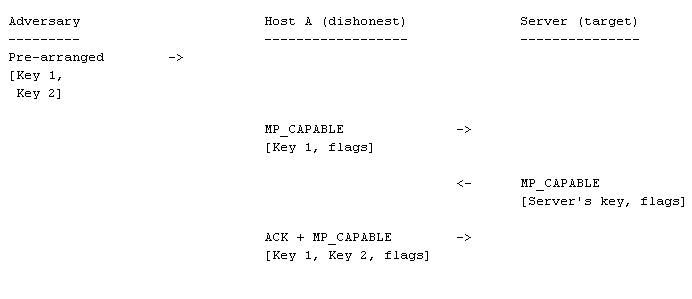
\includegraphics[scale = 0.6]{Figures/mpcapattack.png}
\captionof{figure}{Possible Key Change Attack}
\label{pic:2 cap attack}
\end{minipage} \\ 
%
%\begin{figure}[!t]
%\centering
%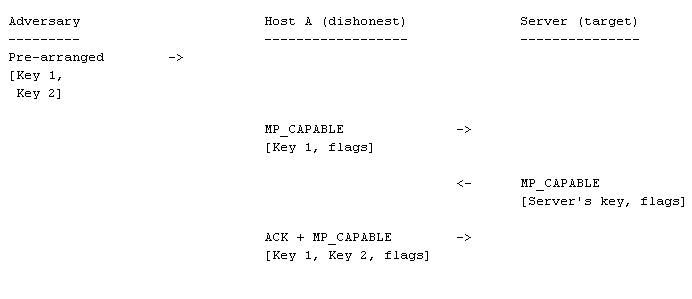
\includegraphics[scale = 0.6]{Figures/mpcapattack.png}
%\caption{Possible Key Change Attack}
%\label{pic:2 cap attack}
%\end{figure}

Unfortunately for our adversary, the authors of the RFC did take this into consideration, the rest of the paragraph reading: ``If the listener acts in this way, however, it MUST generate its key in a way that would allow it to verify that it generated the key when it is echoed in the ACK.''. An implementation conforming to the standard should therefore be equipped to deal with this situation, probably by ignoring it, and of course no one would dare to forget implementing a single guideline of the standard. However, a network operator may still desire to be informed that someone made a futile attempt at breaking the protocol. Let us use the notice framework once again to signal this behavior.\\

To handle the problem, we will create a new \texttt{Pending\_conn} record composed of two booleans and two counts. The booleans are true if the originator's (resp. responder's) key was seen during the original SYN (resp. SYN+ACK). The counts each hold one of the host's key. We will also need an additional table which will map a connection (identified by the address/port four-tuple) to the related \texttt{Pending\_conn}. The issue is confined to MP Capable options only. After adding the new notice type (MP\_key\_change) to the framework, we will therefore head back to the \texttt{mp\_capable} event handler. When receiving an MP Capable SYN, we will create a new entry in the pending table, containing Host A's key. When we receive the SYN+ACK, we must check whether an entry for the connection already exists (it might not if Bro did not see the SYN packet). If the entry exists, we add Host B's key to it, otherwise we create a new entry with B's key only. Finally, when we receive the final ACK, we check to make sure the keys received match those in the table. We only check the values we have seen since, again, Bro may have missed certain packets. Should one or both keys be different from what was expected, a notice is raised. In any case, the pending entry is deleted for memory management reasons. \\

As in the previous section, the notice hook will not perform any action other than printing out the message.

\section{Unknown Join Detection}
The notice for unknown joins deserve a brief mention as it might not do what one might expect. In its current form, it is raised when a Join of length 16 (SYN+ACK) is seen, but the destination address does not belong to any known MPTCP connection in Bro's memory. The important thing to remember is that it is therefore raised when the responder is replying, indicating that both hosts using the subflow appear to know it, even if Bro does not. \\

That being said, the notice does serve a certain purpose since it indicates that some address advertisement was obviously missed. Usually, this will be due to one of three scenarios: \\

\begin{enumerate}
\item The address advertisement was done on a path that does not go through the IDS. In this case, it might indicate a poor design of the network from a security point of view.
\item The packet header was modified along the path, making the destination address observed in the Join different from the one that was advertised by the destination. This implicitly reveals the presence of middle boxes along the path.
\item The advertisement was done before Bro was launched or was not captured if using a packet capture.
\end{enumerate}


\section{Join Flooding}
The initiator of a join first sends the token identifying the connection he wishes to join, along with a random number used for authentication. The receiver must reply with his own random number, and more importantly, a HMAC (truncated to 64 bits) of the two random numbers. This means that the receiver is actually the first host which has to perform a cryptographic operation. The token serves as a form of protection against flooding the server with join demands. Indeed, if a host receive a join SYN with a token it does not know, it should reply with an rst and no calculation is performed. This is stated in the standard \cite{rfc6824}: ``Although calculating an HMAC requires cryptographic operations, it is believed that the 32-bit token in the MP\_JOIN SYN gives sufficient protection against blind state exhaustion attacks''.\\

However, figure \ref{pic:join flood} shows a potentially problematic scenario. Here, we see an adversary begin a legitimate MPTCP connection, obtaining a regular key allowing him to compute the token for this session. Later, perhaps after the server has advertised a second address, the adversary begins flooding the server with Join attempts. His token is valid, forcing the server to compute the HMAC. Of course, the adversary need not reply to these HMACs since he does not intend to use the new subflows. \\

\begin{figure}[!t]
\centering
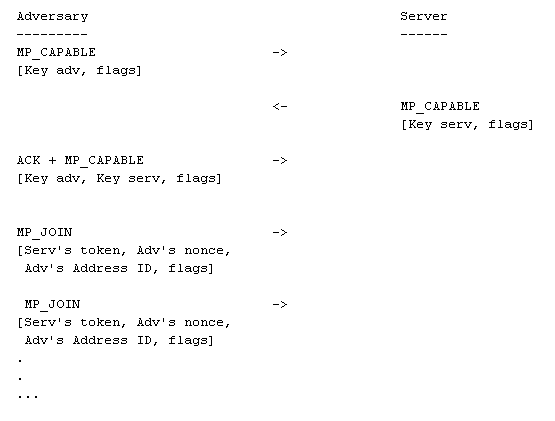
\includegraphics[scale = 0.75]{Figures/joinflood.png}
\caption{Potential Attack on the Join Authentication}
\label{pic:join flood}
\end{figure}

Should this attack be possible, could we detect it? A typical IDS would probably detect this attack as a standard SYN flooding since fundamentally, it is one. However, we are still interested in detecting for what it really is. The first reason is simply to detect MPTCP potentially playing a part in an attack. The second is that the attack is asymmetrical in the sense that a small request causes a heavy computation. An attacker might purposefully lower the sending rate to the point where an automatic SYN flooding detection would not register it, while still sufficiently disturbing the target due to the cryptographic operations.\\

We therefore propose a simple method to detect excess MP Join messages. For every receiver we see, we count the number of MP Join SYN packets he gets. If the number exceeds a set threshold, we raise an \texttt{MP\_join\_flood} notice. At set time intervals, all the counters are reset. The notice that is raised is slightly more complex than those we have used up until now. In addition to the traditional note, msg, and conn fields, we add an identifier and a suppress\_for value. Together, these attributes will ensure that the notice for a given address is only raised once per time interval. This is needed because, once a SYN causes the counter to exceed the threshold, every other SYN thereafter would also cause the notice to be raised. \\

This method of detection is similar to that used by the TCP SYN flood detection script that shipped with the early versions of Bro \cite{synflood}. It was adapted to run smoothly on a packet-trace given that the real-time rate at which packets arrive is usually a key factor in such an attack. Another issue with both the original TCP and this MPTCP detection methods is the use of a static threshold.

